\begin{figure}[htp]
	\subcaptionbox{Sequential}[0.45\textwidth]
	{
		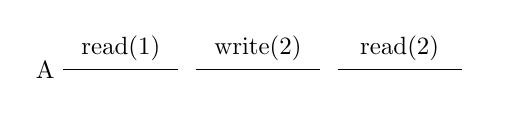
\begin{tikzpicture}[scale=0.9, transform shape] 
		\node (x1)  {A};
		\node (x2) [right of=x1,xshift=1cm]{};
		\draw (x1) -- node[above]{read(1)} (x2);
		\node(x3)[right of=x2,xshift=-1cm]{};
		\node(x4) [right of=x3,xshift=1cm]{};
		\draw (x3) -- node[above]{write(2)} (x4);
		
		\node(x5)[right of=x4,xshift=-1cm]{};
		\node(x6) [right of=x5,xshift=1cm]{};
		\draw (x5) -- node[above]{read(2)} (x6);
		\end{tikzpicture}
	}
	%\quad
	\subcaptionbox{Concurrent - linearizable}[0.45\textwidth]
	{
		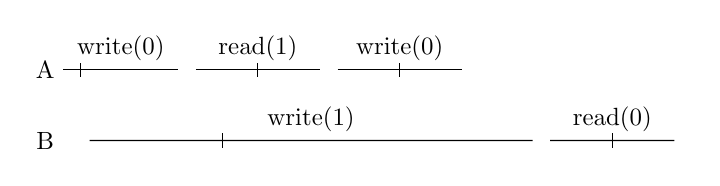
\begin{tikzpicture}[scale=0.9, transform shape] 
		\node (x1) {A};
		\node (x2) [right of=x1,xshift=1cm]{};
		\draw (x1) -- node[above]{write(0)} (x2);
		\draw (0.5,-0.1) -- (0.5,+0.1);
		
		\node(x3)[right of=x2,xshift=-1cm]{};
		\node(x4) [right of=x3,xshift=1cm]{};
		\draw (x3) -- node[above]{read(1)} (x4);
		\draw (3,-0.1) -- (3,+0.1);
		
		\node(x5)[right of=x4,xshift=-1cm]{};
		\node(x6) [right of=x5,xshift=1cm]{};
		\draw (x5) -- node[above]{write(0)} (x6);
		\draw (5,-0.1) -- (5,+0.1);
		
		\node(B)[below of=x1]{B};
		\node(x7)[below of=x1,xshift=0.5cm]{};
		\node(x8) [right of=x7,xshift=5.5cm]{};
		\draw (x7) -- node[above]{write(1)} (x8);
		\draw (2.5,-1.1) -- (2.5,-0.9);
		
		\node(x9)[right of=x8,xshift=-1cm]{};
		\node(x10) [right of=x9,xshift=1cm]{};
		\draw (x9) -- node[above]{read(0)} (x10);
		\draw (8,-1.1) -- (8,-0.9);
		
		\end{tikzpicture}
	}
%%%%%%%%%%%%%%
\\
%%%%%%%%%%%%%%
%%%%%%%%%%%%%%
\\
%%%%%%%%%%%%%%
\begin{center}
	\subcaptionbox{Concurrent - not linearizable}
	{
		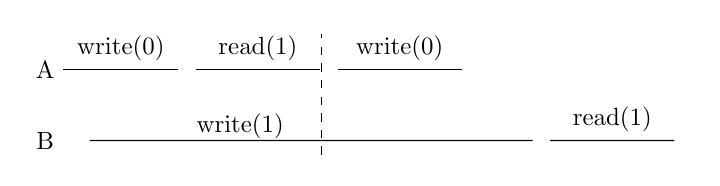
\begin{tikzpicture}[scale=0.9, transform shape] 
		\node (x1) {A};
		\node (x2) [right of=x1,xshift=1cm]{};
		\draw (x1) -- node[above]{write(0)} (x2);
		
		\node(x3)[right of=x2,xshift=-1cm]{};
		\node(x4) [right of=x3,xshift=1cm]{};
		\draw (x3) -- node[above]{read(1)} (x4);
		\draw[dashed] (3.9,-1.2) -- (3.9,+0.5);
		
		\node(x5)[right of=x4,xshift=-1cm]{};
		\node(x6) [right of=x5,xshift=1cm]{};
		\draw (x5) -- node[above]{write(0)} (x6);
		
		\node(B)[below of=x1]{B};
		\node(x7)[below of=x1,xshift=0.5cm]{};
		\node(x8) [right of=x7,xshift=5.5cm]{};
		\draw (x7) -- node [above, xshift=-1cm,yshift=-0.1cm] {write(1)} (x8);
		
		\node(x9)[right of=x8,xshift=-1cm]{};
		\node(x10) [right of=x9,xshift=1cm]{};
		\draw (x9) -- node[above]{read(1)} (x10);
		
		\end{tikzpicture}
	}
	\caption{A sample history of an object \label{fig:linearizability}}
\end{center}
\end{figure}